\section{Preliminaries} \label{sec:prelim}

The DCEL \cite{muller_finding_1978} structure is used to represent an embedding of a planar subdivision in the plane. It provides efficient manipulation of the geometric and topological features of spatial objects (polygons, lines, and points) using \textit{faces}, \textit{edges}, and \textit{vertices}, respectively. A DCEL uses three tables (relations) to store records for the faces, edges, and vertices, respectively. 

An important characteristic is that all these records are defined using edges as the main component (thus termed an edge-based structure). Examples appear in Tables \ref{tab:vertices}-\ref{tab:hedges}, with the subdivision depicted in Figure \ref{fig:dcel_example}.

\begin{table*} \label{tab:records}
\begin{minipage}{0.49\textwidth}
    \small
    \centering
    \caption{Vertex records.}\label{tab:vertices}
    \begin{tabular}{c c c}
        \toprule
        vertex & coordinates & incident edge \\
        \midrule
        a      & (0,2)  & $\vec{ba}$ \\
        b      & (2,0)  & $\vec{db}$ \\
        c      & (2,4)  & $\vec{dc}$ \\
        \vdots & \vdots & \vdots     \\
        \bottomrule
    \end{tabular}
\end{minipage}\hfill % maximize the horizontal separation
\begin{minipage}{0.49\textwidth}
    \small
    \centering
    \caption{Face records.}\label{tab:faces}
    \begin{tabular}{c c c} 
        \toprule
             & boundary  & hole\\
        face & edge      & list\\
        \midrule
        $f_1$ & $\vec{ab}$ & $nil$ \\
        $f_2$ & $\vec{fe}$ & $nil$ \\
        $f_3$ & $nil$      & $nil$ \\
        \bottomrule
    \end{tabular}
\end{minipage}
\end{table*}

\begin{table*} 
\begin{minipage}{\textwidth}
    \small
    \centering
    \caption{Half-edge records.}\label{tab:hedges}
    \begin{tabular}{c c c c c c} 
        \toprule
        half-edge & origin & face & twin & next & prev \\
        \midrule
        $\vec{fe}$ & f & $f_2$  & $\vec{ef}$ & $\vec{ec}$ & $\vec{df}$ \\
        $\vec{ca}$ & c & $f_1$  & $\vec{ac}$ & $\vec{ab}$ & $\vec{dc}$ \\
        $\vec{db}$ & d & $f_3$  & $\vec{bd}$ & $\vec{ba}$ & $\vec{fd}$ \\
        \vdots     & \vdots & \vdots & \vdots     & \vdots     & \vdots     \\
        \bottomrule
    \end{tabular}
\end{minipage}
\end{table*}

An edge corresponds to a straight line segment shared by two adjacent faces (polygons). Each of these two faces will use this edge in its description; to distinguish, each edge has two \textit{half-edges}, one for each orientation (direction). It is important to note that half-edges are oriented counter-clockwise inside each face (Figure \ref{fig:dcel_example}). A half-edge is thus defined by its two vertices, one called the \textit{origin} vertex and the other the \textit{target} vertex, clearly specifying the half-edge's orientation (origin to target). Each half-edge record contains references to its origin vertex, its face, its \textit{twin} half-edge, as well as the next and previous half-edges (using the orientation of its face); see Table \ref{tab:hedges}. These references are used as keys to the tables that contain the referred attributes. 

Figure \ref{fig:dcel_example} shows half-edge $\overrightarrow{fe}$, its \textit{twin($\overrightarrow{fe}$)} (which is half-edge $\overrightarrow{ef}$), the \textit{next($\overrightarrow{fe}$)} (half-edge $\overrightarrow{ec}$) and the \textit{prev($\overrightarrow{fe}$)} (half-edge $\overrightarrow{df}$). Note the counter-clockwise direction used by the half-edges comprising face $f_2$. The \textit{incidentFace} of a half-edge corresponds to the face that this edge belongs to (for example, \textit{incidentFace}($\overrightarrow{fe}$) is face $f_2$). 
In addition, we note a couple of special half-edges. 
\textit{Dangles} are the half-edges with one or both ends not incident on another half-edge endpoint. Half-edge \textit{$\overrightarrow{fj}$} and its twin are both considered dangle edges.
\textit{Cut-Edges} are the half-edges connected at both ends but do not form part of a polygon. 
The half-edge \textit{$\overrightarrow{dg}$} and its twin are considered cut-edges.

% \textbf{\color{red} TODO: Add to this part a description of the new figure 1 showing Dangle and Cut edge of DCEL \color{blue}[DONE] See above.}

Each vertex corresponds to a record in the vertex table (see Table \ref{tab:vertices}) that contains its coordinates as well as one of its incident half-edges. An incident half-edge is one whose target is this vertex. Any of the incident edges can be used; the rest of a vertex's incident half-edges can be found easily following the next and twin half-edges.

Finally, each record in the faces table contains one of the face's half edges to describe the polygon's outer boundary (following this face's orientation); see Table \ref{tab:faces}. All other half-edges for this face's boundary can be easily retrieved following the next half-edges in orientation order. In addition to regular faces, there is one face that covers the area outside all faces; it is called the  \textit{unbounded} face (face $f_3$ in Figure \ref{fig:dcel_example}). Since $f_3$ has no boundary, its boundary edge is set to \textit{nil} in Table \ref{tab:faces}.

Note that polygons can contain one or more \textit{holes} (a hole is an area inside the polygon that does not belong to it). Each such hole is described by one of its half-edges; this information is stored as a list attribute (hole list) in the faces table where each element of the list is the half-edge's id which describes the hole. Note that in Table \ref{tab:faces}, this list is empty as there are no holes in any of the faces in the example of Figure \ref{fig:dcel_example}. 

An important advantage of the DCEL structure is that a user can combine two DCELs from different layers over the same area (e.g., the census tracts from two different years) and compute their \textit{overlay}, which is a DCEL structure that combines the two layers into one. Other operators, like the intersection, difference, etc., can then be computed from the overlay very efficiently. Given two DCEL layers $S_1$ and $S_2$, a face $f$ appears in their overlay  $OVL(S_1, S_2)$ if and only if there are faces $f_1$ in $S_1$ and $f_2$ in $S_2$ such that $f$ is a maximal connected subset of $f1 \cap f2$ \cite{berg_computational_2008}. This property implies that the overlay $OVL(S_1, S_2)$ can be constructed using the half-edges from $S_1$ and $S_2$. 

The sequential algorithm \cite{fogel_cgal_2012} to construct the overlay between two DCELs first extracts the half-edge segments from the half-edge tables and then finds intersection points between half-edges from the two layers (using a sweep line approach) \cite{berg_computational_2008}. The intersection points found will become new vertices of the resulting overlay. If an existing half-edge contains an intersection point, it is split into two new half-edges. Using the list of outgoing and incoming half-edges for the newly added vertices (intersection points), the algorithm can compute the attributes for the records of the new half-edges. For example, the list of outgoing and incoming half-edges at each new vertex will be used to update the next, previous, and twin pointers. Finally, the records of the faces and the vertices tables are updated with the new information. 

\begin{figure}
    \centering
    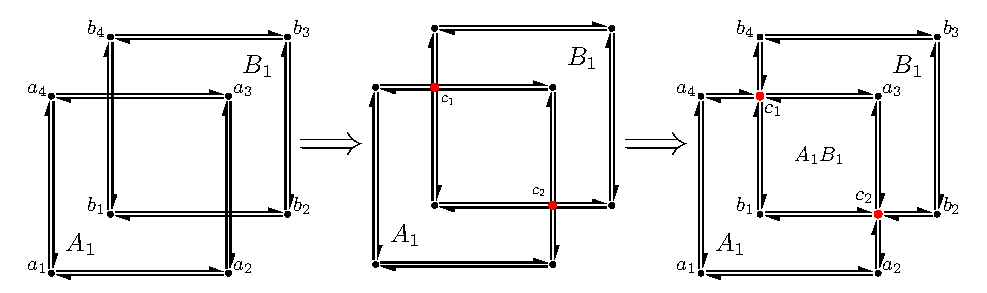
\includegraphics[width=\linewidth]{chapter2/dcel2}
    \caption{Sequential computations of an overlay of two DCEL layers.}\label{fig:dcel_seq}
\end{figure}

Figure \ref{fig:dcel_seq} illustrates an example of computing the overlay between two DCEL layers with one face each ($A_1$ and $B_1$ respectively) overlapping the same area. First, intersection points are identified, and new vertices are created in the overlay (red vertices $c_1$ and $c_2$). Then, new half-edges are created around these new vertices. As a result, face $A_1$ is modified (to an L-shaped boundary), as does face $B_1$, while a new face $A_1B_1$ is created. Since this new face is the intersection of the boundaries of $A_1$ and $B_1$, its label contains the concatenation of both face labels. By convention \cite{berg_computational_2008}, even though $A_1$ changes its shape, it does not change its label since its new shape is created by its intersection with the unbounded face of $B_1$; similarly, the new shape of $B_1$ maintains its original label. These labels are crucial for creating the overlay (and the operators it supports) as they are used to identify which polygons overlap an existing face.

Once the overlay structure of two DCELs is computed, queries like their intersection, union, difference, etc. (Figure \ref{fig:dcel_operators}) can be performed in linear time to the number of faces in the overlay. The space requirement for the overlay structure remains linear to the number of vertices, edges, and faces. Since an overlay is itself a DCEL, it can support the traditional DCEL operations (e.g., find the boundary of a face, access a face from an adjacent one, visit all the edges around a vertex, etc.)

\begin{figure}
    \centering
    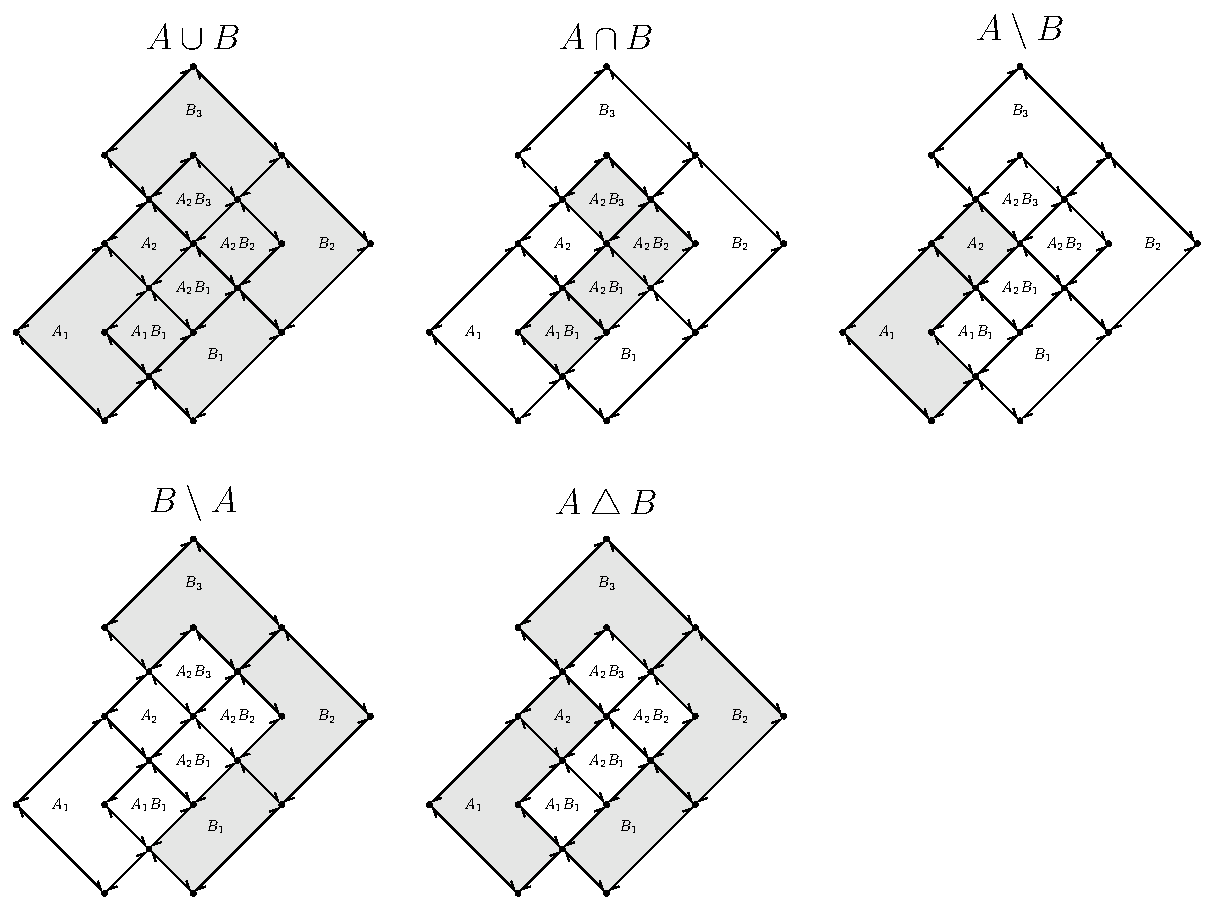
\includegraphics[width=0.8\textwidth]{chapter2/dcel_operators.pdf}
    \caption{Examples of overlay operators supported by DCEL; results are shown in gray.}
    \label{fig:dcel_operators}
\end{figure}

\section{Scalable Overlay Construction} \label{sec:methods}

This section presents the construction of overlay DCELs, assuming only polygons as input without scattered line segments. The overlay computation depends on the size of the input DCELs and the size of the resulting overlay. The DCEL of a planar subdivision $S_1$ has size $O(n_1)$ where $n_1$ = $\Sigma (vertices_1 + edges_1 + faces_1$).  The sequential algorithm constructing the overlay of $S_1$ and $S_2$ takes $O(n \log n + k \log n)$ time, where $n = n_1 + n_2$ and $k$ is the size of their overlay.  Note that $k$ depends on how many intersections occur between the input DCELs, which can be very large \cite{berg_computational_2008}. 

While the sequential algorithm is efficient with small DCEL layers, it suffers when the input layers are large and have many intersections. For example, creating the overlay between the DCELs of two census tracts (from years 2000 and 2010) from California (each with 7K-8K polygons and 2.7M-2.9M edges) took about 800sec on an Intel Xeon CPU at 1.70GHz  with 2GB of memory (see Section \ref{sec:experiments}). With DCELs corresponding to the whole US, the algorithm crashed. 

Nevertheless, the overlay computation can take advantage of \textit{\textbf{partitioning}} (and thus parallelism) by observing that the edges in a given area of one input layer can only intersect with edges from the same area in the other input layer. One can thus spatially partition the two input DCELs 
%using a spatial index (or grid) 
and then compute the overlay within each cell; such computations are independent and can be performed in parallel. While this is a high-level view of our scalable approach, there are various challenges, including how to deal with edges that cross cells, how to manage the extra complexity introduced by \textit{orphan} holes (i.e., when holes and their polygons are in different cells), how and where to combine partition overlays into a global overlay, as well as how to balance the computation if one layer is much larger than the other. 

\subsection{Partition Strategies} \label{sec:pstrategies}
While a simple grid could be used to divide the spatial area, our early experiments demonstrated that this approach leads to unbalanced cells, with some containing significantly more edges than others, negatively impacting overall performance.

Therefore, an advanced partitioning strategy is better since it adapts to skewed spatial distributions and helps assign a similar number of edges to each cell. In particular, we used two partitioning strategies, one based on the quadtree (i.e. space-oriented) and one on the kd-tree (i.e. data-oriented) indexes.

Note that such tree-based data partitioning involves shuffling all edges; this however, happens only once.
Our experimental evaluation (see Section \ref{sec:comparison}) shows that the data-oriented approach leads to better performance. Nevertheless, in describing the various challenges (orphan cells and holes, overlay evaluation, and optimizations) we use the quadtree-based partition since its well-defined space-oriented partitioning makes the presentation easier.

\subsubsection{Quadtree Partition Strategy}\label{sec:strategy}
The main idea of the quadtree partition strategy is to split the area covered by the input layers into non-overlapping cells, which can then be processed independently. 
A quadtree data structure follows a space-oriented approach, given that it does not consider each cell's content at the moment of a possible split. 
The overall approach can be summarized in the following steps: (i) Partition the input layers into the index cells and build local DCEL representations of them at each cell, and (ii) Compute the overlay of the DCELs at each cell. Overlay operators and other functions can be run over the local overlays, and local results are collected to generate the final answer.  

Note that each input layer is given as a sequence of polygon edges, where each edge record contains the coordinates of the edge's vertices (origin and target vertex) as well as the polygon id and a hole id in the case that an edge belongs to a hole inside of a polygon. We assume there are no overlapping or stacked polygons in the dataset. 

To quickly build the partitioning quadtree structure, we build a quadtree from a sample taken from the edges of each layer (1\% of the total number of edges in that layer). We then use the leaves of that quadtree as the cells (partitions) of the partitioning scheme. These cells will be used to assign the edges of each input layer. Populated cells are then distributed to the available nodes for processing the overlay operations. 

To support the creation of the quadtree we use the sampling functionalities provided in the Apache Sedona, an extension available on the Apache Spark platform. It allows the user to provide a parameter for the number of quadtree leaves; using this parameter as an approximation, it builds a quadtree; it should be noted that the actual number of leaves created is typically larger than the parameter provided by the user. The number of user-requested leaves and the size of the sample are used to compute the maximum number of entries per node (capacity) during the construction of the tree.  If the node capacity is exceeded, the node is divided into four child nodes with an equal spatial area, and its data is distributed among the four child nodes.  If any child node has exceeded its capacity, it is further divided into four nodes recursively and so on, until each node holds at most its computed \textit{capacity}.

After creating the quadtree from the sample, we use its leaf nodes as the partitioning cells for each layer. Each input layer file is then read from the disk, and \textit{all} its edges are inserted into the appropriate cells of the partitioning structure. Note that the partitioning structure created from the sample is now fixed; no more cells are created when the layer edges are assigned to cells. In the rest, we use the term cell and partition interchangeably.

For this approach to work, it is important that each cell can compute its two DCELs independently. An edge can be fully contained in a cell, or it can intersect the cell's boundary. In the second case, we copy this edge to all cells where it intersects, but within each cell, we use the part of the edge that lies fully inside the cell. Figure \ref{fig:partition_strategy} shows an example where four cells and two edges of the upper polygon from layer A cross the cell borders. Such edges are clipped at the cell borders, introducing new edges (e.g., edges $\alpha^{\prime}$ and $\alpha^{\prime \prime}$ in the Figure \ref{fig:partition_strategy}).
Similarly, a polygon that crosses over a cell is clipped to the cell by introducing \textit{\textbf{artificial}} edges on the cell's border (see face $A_2$ in cell 3 of Figure \ref{fig:partition_strategy}). Such artificial edges are shown in red in the figure. This allows for the creation of a smaller polygon that is contained within each cell. 

For example, polygon $A_2$ is clipped into four smaller polygons as it overlaps all four cells. The clipping of edges and polygons ensures that each cell has all the needed information to complete its DCEL computations. As such computations can be performed independently, they are sent to different worker nodes to be processed in parallel. The assignment is delegated to the distributed framework (i.e., Apache Spark). 

\begin{figure}
    \centering
    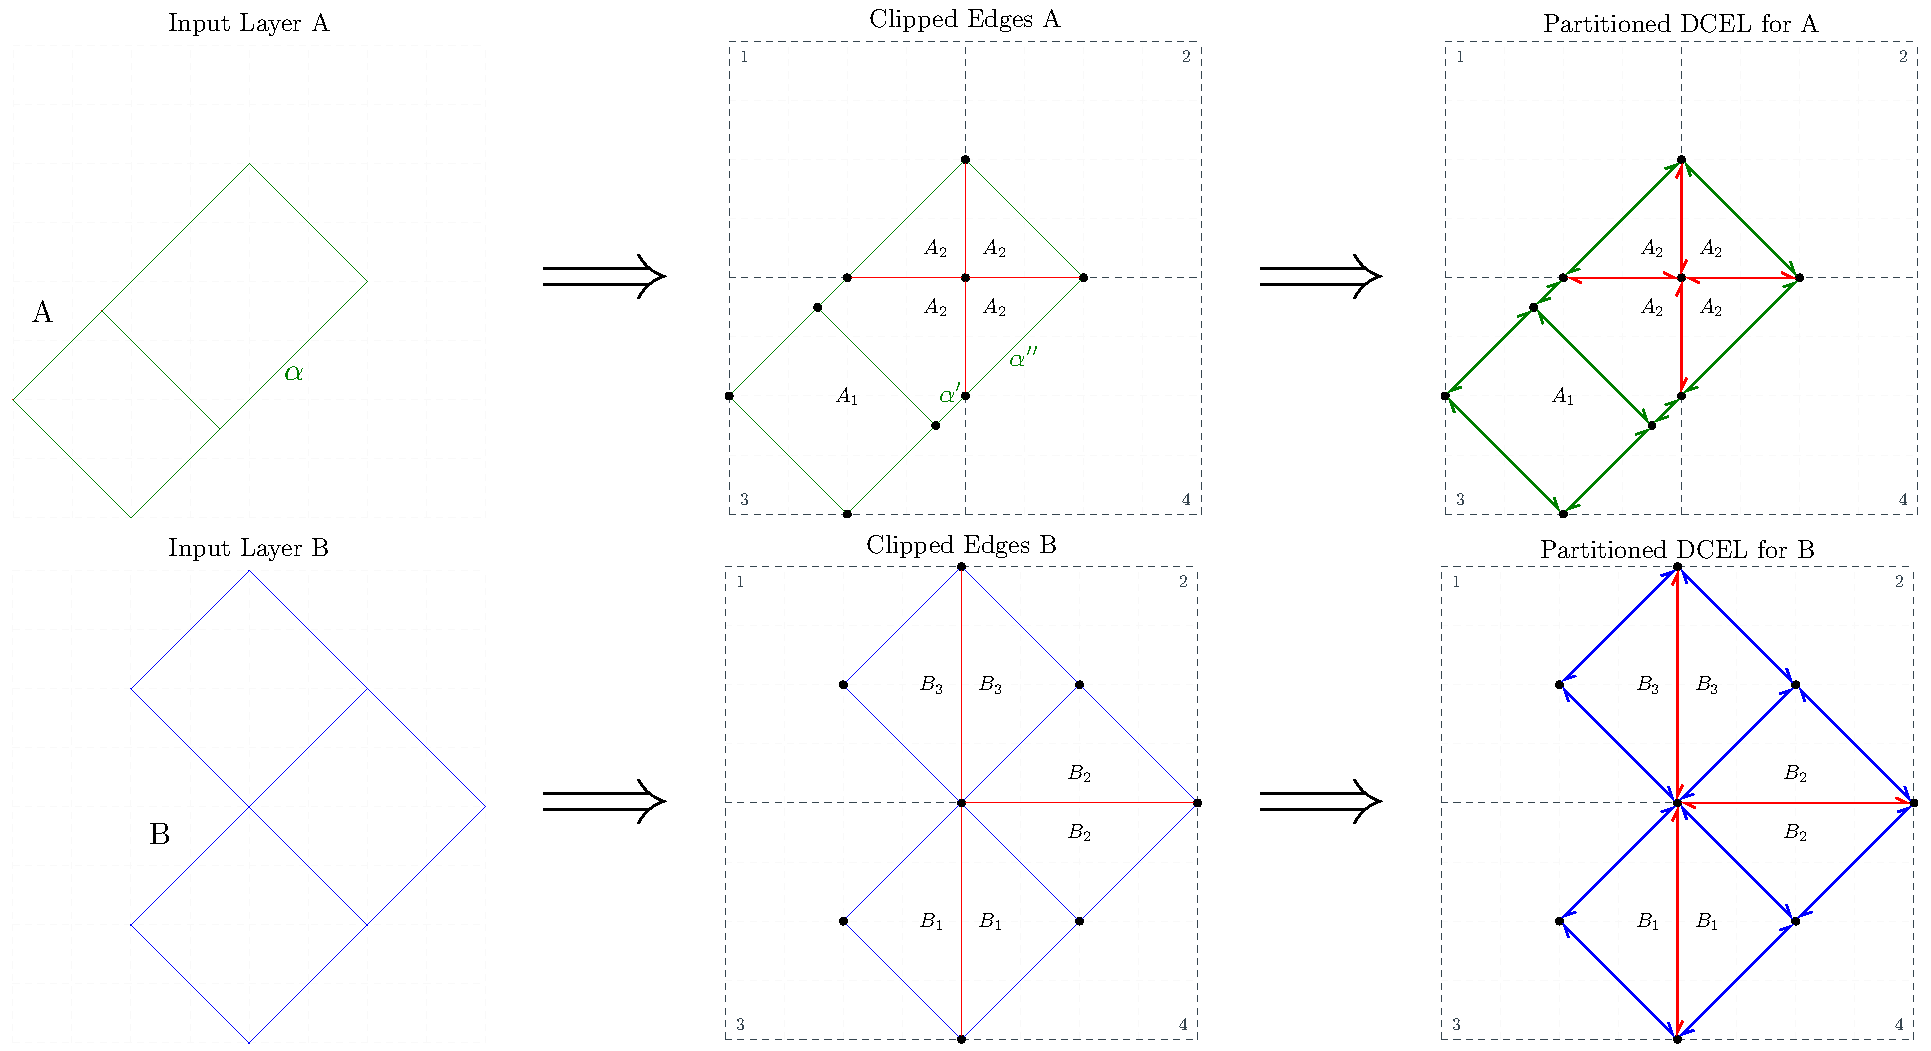
\includegraphics[width=\textwidth]{chapter2/polygons_parted}
    \caption{Partitioning example using input layers A and B over four cells.} \label{fig:partition_strategy}
\end{figure}

Once a cell is assigned to a worker node, the sequential algorithm is used to create a DCEL for each layer (using the cell edges from that layer and any artificial edges, vertices, and faces created by the clipping procedures above) and then compute the corresponding (local) overlay for this cell. Using the example from Figure \ref{fig:partition_strategy}, Figure \ref{fig:overlay_partition} depicts an overview of the process for creating a local overlay DCEL inside cell 2. Similarly, Figure \ref{fig:distributed_dcel} shows all local overlay DCELs computed at each cell (artificial edges are shown in red). 

\begin{figure}
    \centering
    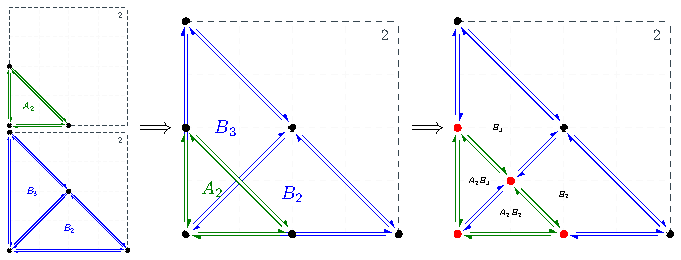
\includegraphics[width=0.9\linewidth]{chapter2/overlay_partition.pdf}
    \caption{Local overlay DCEL for cell 2.}\label{fig:overlay_partition}
\end{figure}

\begin{figure}
    \centering
    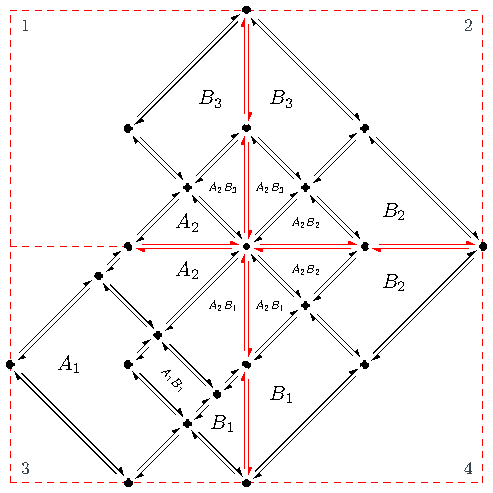
\includegraphics[width=0.6\linewidth]{chapter2/distributed_dcel.pdf}    
    \caption{Result of the local overlay DCEL computations.}\label{fig:distributed_dcel}
\end{figure}

%%%
% Orphan cell and orphan hole problems...
%%%
Nevertheless, the partitioning creates two problems (not present in the sequential environment) that need to be addressed. 
The first is the case where a cell is empty; it does not intersect with (or contain) any regular edge from either layer. A regular edge is not part of a hole.
This empty cell does not contain any label, and thus, we do not know which face it may belong to. We term this as the \textbf{\textit{orphan cell}} problem.
An example is shown in Figure \ref{fig:orphan_cells}, which depicts a face (from one of the input layers) whose boundary goes over many quadtree cells; orphan cells are shown in grey. 

Note that an orphan cell may contain a hole (see Figure \ref{fig:orphan_cells}). In this case, the original label of the face where the hole belongs (and reported in the hole's edges) may have changed during the overlay computation (because it overlapped with a face from the other layer). However, this new label has not been propagated to the hole edges.
We term this as the \textbf{\textit{orphan hole}} problem. For simplicity, we focus on the case where a hole is within one orphan cell, but in the general case, a hole can split among many such cells.

The issue with both `orphan' problems is the missing labels. In section \ref{sec:anomalies}, we propose an algorithm that correctly labels an orphan cell. If this cell contains a hole, the new label is also used to update the hole edges. 

\begin{figure}
    \centering
    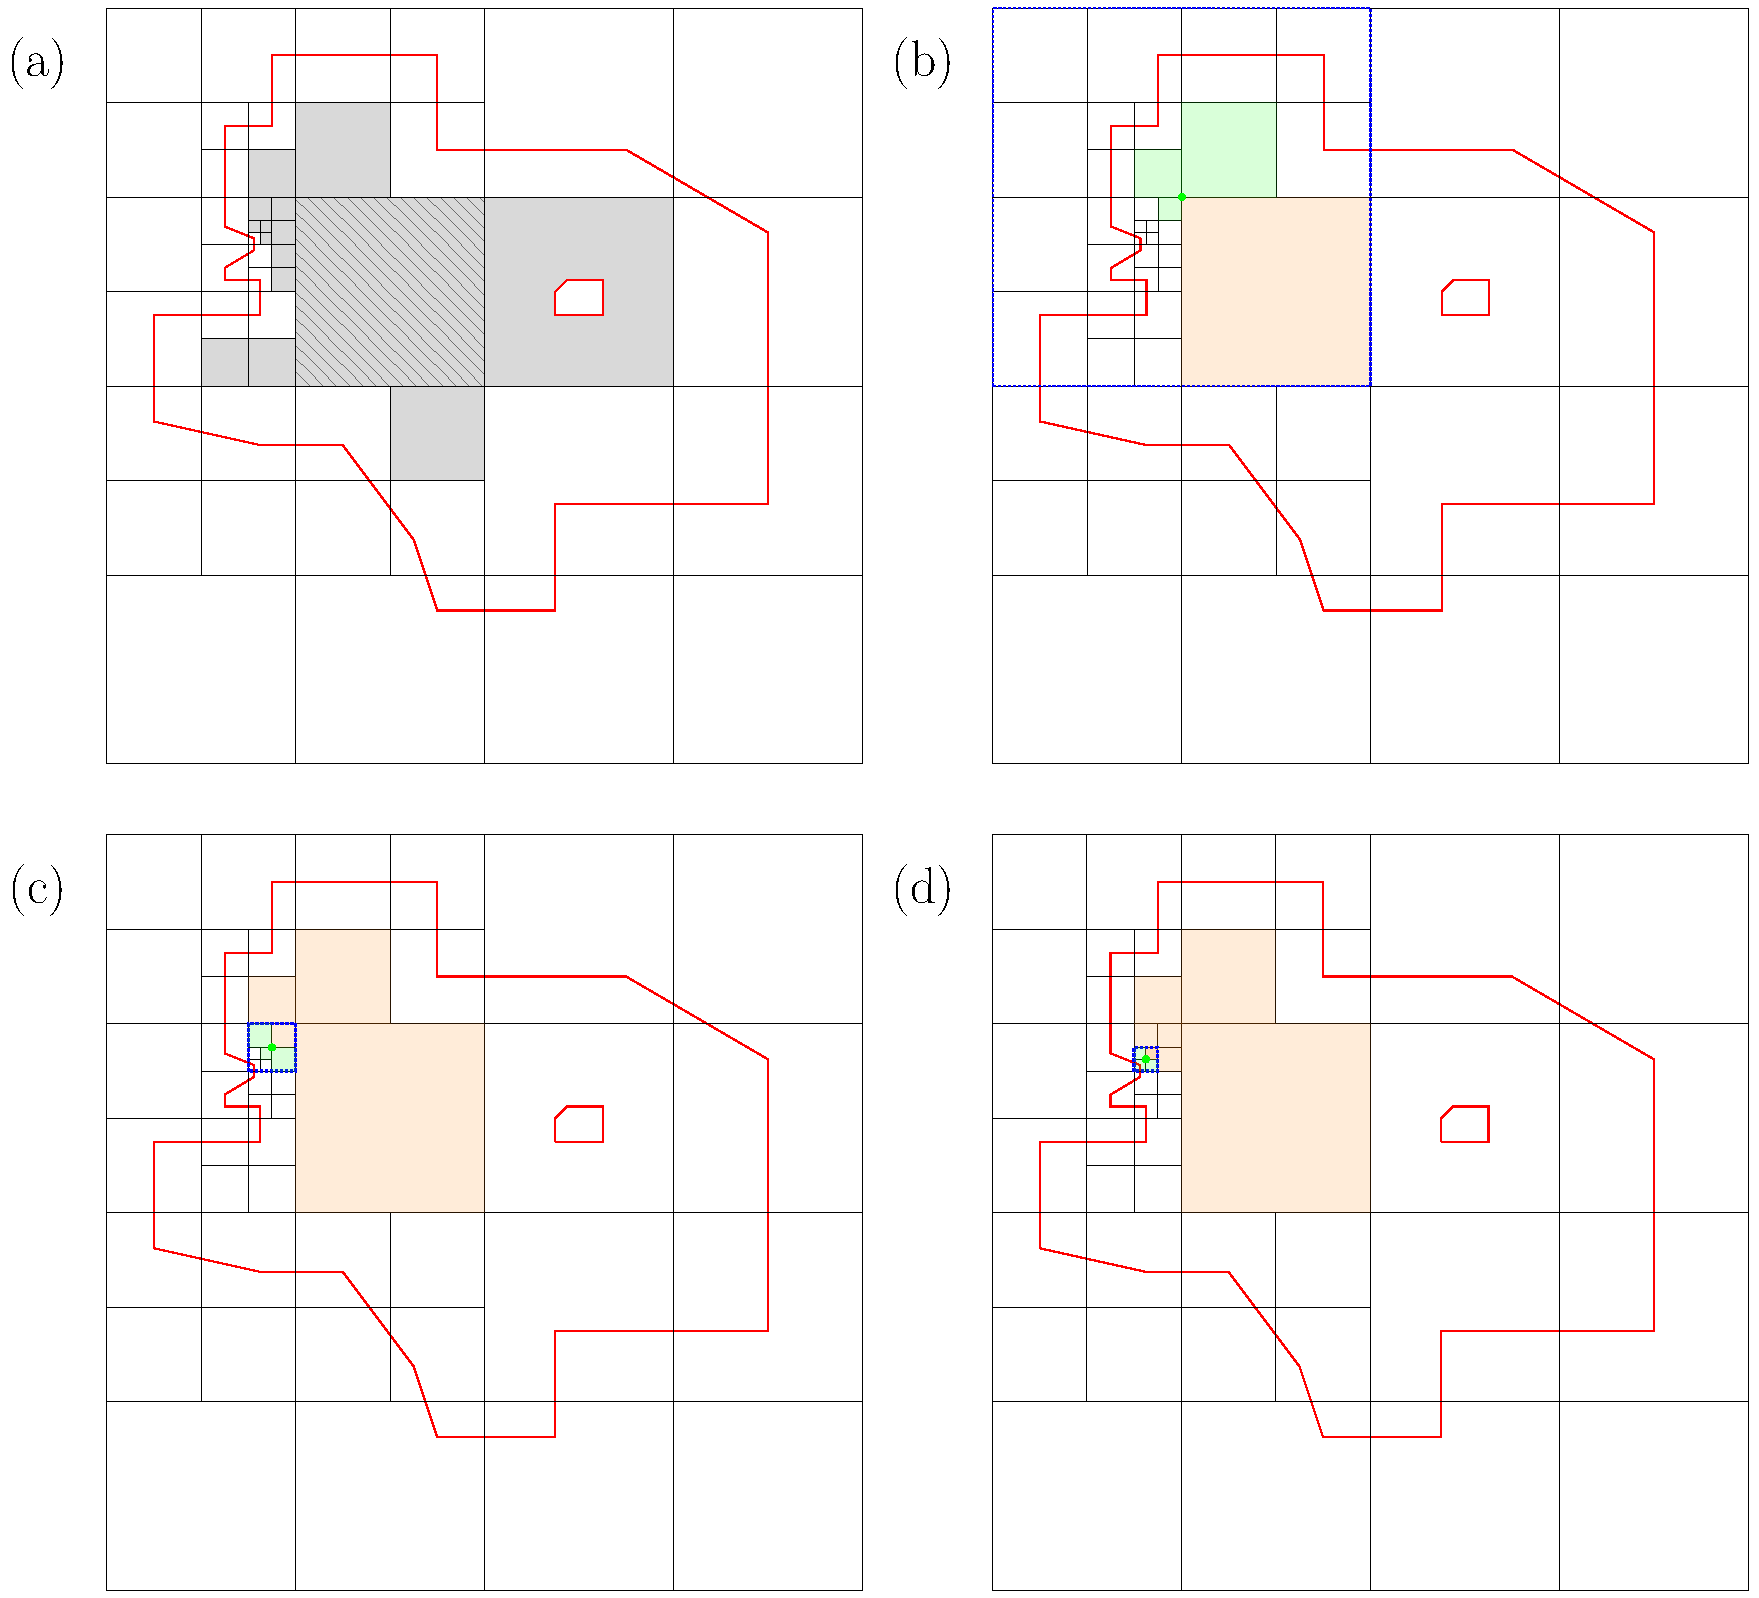
\includegraphics[width=\linewidth]{chapter2/orphan_cells.pdf}    
    \caption{(a) Empty cell and hole examples; (b)-(c)-(d) show three iterations of the proposed solution.} \label{fig:orphan_cells}
\end{figure}

\subsubsection{Kd-tree Partition Strategy} \label{sec:kdtreestrategy}


%A quadtree data structure follows a space-oriented approach, given that it does not consider each cell's content at the moment of a possible split. 
%However, their use and simplicity help as an initial approach. 
The kd-tree based partitioning is a data-oriented approach because it sorts and picks the middle point inside a cell to locate the split of the future children. %Given these characteristics, a quadtree is more prone to introduce an empty cell, which could lead to the `orphan' problems described in section \ref{sec:anomalies}.

%To measure the impact on the performance of a different partitioning approach, our implementation was updated to create a kd-tree from a sample of the input data. 
Building and populating the kd-tree partitioning follows a procedure similar to that of the quadtree, by first building a kd-tree from a sample of the input data.
1\% of the input data is used to build a kd-tree and extract the tree's structure. 
The leaves of this structure are the partition's cells. 
We feed the input data into the generated kd-tree structure to assign each edge to the leaf cell that has the edge within its boundaries.  
After the partitioning is done, the construction of the local DCELs for each layer and the overlay operation is performed in each local cell in the same fashion as described in section \ref{sec:strategy}. 
% It is expected that the different approach provided by the kd-tree could help in the organization and transmission of the data and the overlay performance.
% Then, a shuffle is performed in the data assigning a new worker node depending of the partition identifier. All data which lie in the same kd-tree leaf will finish in the same worker node.  


%\textbf{\color{red} TODO: this is a placeholder for the writing of the new contribution of kd-tree partitioning strategy. It has to follow the same style as the Quadtree strategy section. \color{blue}[Work in progress...]}

\subsection{Labeling Orphan Cells and Holes} \label{sec:anomalies}

%{\color{blue} This section details the process of detecting and labeling orphan cells and holes in input polygons.
%For simplicity of presentation, and without loss of generality, the section starts with discussing the labeling process in the case of quadtree partitioning.
%Then, we discuss the changes when kd-tree partitioning is employed.

%}

%\vspace{4pt}

%\noindent \textbf{Labeling with quadtree partitioning.}
Assuming a quadtree-based partitioning, to find the label of an orphan cell, we propose an algorithm that recursively searches the space around the orphan cell until it identifies a nearby cell that contains an edge(s) of the face that includes the orphan cell and thus acquire the appropriate label information. The quadtree index accommodates this search. Two observations are in order: (1) each cell is a leaf of the quadtree index (by construction), and (2) each cell has a unique id created by the way this cell was created; this id effectively provides the \textit{lineage} (unique path) from the quadtree root to this leaf.

Recall that the root has four possible children (typically numbered as 0,1,2,3 corresponding to the four children NW, NE, SW, and SE). The lineage is the sequence of these numbers in the path to the leaf. For example, the lineage for the shaded orphan cell in Figure \ref{fig:orphan_cells}(a) is 03. Further, note that the quadtree is an unbalanced structure, having more deep leaves where there are more edges. Thus, higher leaves correspond to larger areas, and deeper leaves correspond to smaller areas (since a cell split is created when a cell has more edges than a threshold). After identifying an orphan cell, the question is where to search for a cell containing an edge. The following Lemma applies:

\begin{lemma}\label{lem:cells}
Given an orphan cell, one of its siblings at the same quadtree level must contain a regular edge (directly or in its subtree). 
\end{lemma}

This lemma arises from the simple observation that if all three siblings of an orphan cell are empty, then there is no reason for the quadtree to make this split and create these four siblings. Based on the lemma, we know that at least one of the three siblings of the orphan cell can lead us to a cell with an edge. 
However, these siblings may not be cells (leaves). Instead of searching each one of them in the quadtree until we reach their leaves, we want a way to quickly reach their leaves. To do so, we pick the centroid point of the orphan cell's parent (which is also one of the corners of the orphan cell). 

For example, the parent centroid for the orphan cell 03 is the green point in Figure \ref{fig:orphan_cells}(b). We then query the quadtree to identify which cells (leaves, one from each sibling) contain this point. We check whether these cells contain an edge; if we find such a cell, we stop (and use the label in that cell). If all three cells are orphans, we need to continue the search. 
An example appears in Figure \ref{fig:orphan_cells}(b), where all three cells (green in the figure) are also orphans.
We first check if any of these orphan cells is a sibling (has the same parent) of the original cell. In this case that sibling is also a leaf (i.e. it does not have a subtree) and does need to be explored.
The remaining orphans are therefore at a lower level than the original orphan cell, which means they come from a sibling that has been split because of some edge. The algorithm picks any of the remaining orphan cells to continue. In Figure \ref{fig:orphan_cells}(b) all three leaves (green orphan cells) are at a lower level than the original orphan cell. 

One can use different heuristics to pick which of the remaining leaves to use. Below, we consider the case where we use the deepest cell (i.e., the one with the longest lineage) among the leaves. This is because we expect this to lead us to the denser areas of the quadtree index, where there is more chance to find cells with edges. Figure \ref{fig:orphan_cells} shows a three-iteration run of the algorithm. 

During the search process, we keep any orphan cells we discover; after a cell with an edge (non-orphan cell) is found, the algorithm stops and labels the original orphan cell and any other orphan cells retrieved in the search with the label found in the non-orphan cell. Note that if the non-orphan cell contains many labels (because different faces pass through it), we assign the label of the face that contains the original centroid.

The pseudo-code of the search process can be seen in Algorithms \ref{alg:one} and \ref{alg:two}. Another heuristic we used that is not described here is to follow the highest among the three orphan cells; i.e. the one with the shorter lineage since this has a larger area and will thus help us cover more empty space and possibly reach the border of the face faster.

To determine the worst-case performance of the search algorithm, consider that for an orphan cell, the algorithm performs three point quadtree queries to find the sibling leaves containing the centroid. It then selects one of these leaves and repeats the process, querying three points for a new centroid within the siblings of the selected leaf. This causes the algorithm to explore progressively deeper into the quadtree. In the worst case, the longest path in the quadtree could result in a time complexity of $O(N)$. However, in the average case, when the quadtree is balanced, the complexity is logarithmic.

\begin{algorithm}\caption{\textsc{getNextCellWithEdges} algorithm}\label{alg:one}
    \begin{algorithmic}[1]
    \Require a quadtree $\mathcal Q$ and a list of cells $\mathcal M$.
    \Function{ getNextCellWithEdges }{ $\mathcal Q$, $\mathcal M$ }
        \State $\mathcal C \gets $ orphan cells in $\mathcal M$
        \ForEach{ $orphanCell$ in $\mathcal C $ }
            \State initialize $cellList$ with $orphanCell$ 
            \State $nextCellWithEdges \gets nil$
            \State $referenceCorner \gets nil$
            \State $done \gets false$
            \While{ $\neg done$ } 
                \State $c \gets $ last cell in $cellList$ 
                \State $cells, corner \gets \textsc{getCellsAtCorner}(\mathcal Q, c)$ 
                \ForEach{$cell$ in $cells$}
                    \State $nedges \gets$ get edge count of $cell$ in $\mathcal M$ 
                    \If{ $nedges > 0$ }
                        \State $nextCellWithEdges \gets cell$
                        \State $referenceCorner \gets corner$
                        \State $done \gets true$
                    \Else
                        \If{$cell.level < orphanCell.level$}
                            \State add $cell$ to $cellList$
                        \EndIf
                    \EndIf
                \EndFor
            \EndWhile
            \ForEach{ $cell$ in $cellList$ }
                \State \textbf{output}($cell$, \\
                \hspace{2.5cm} $nextCellWithEdges$, $referenceCorner$)
                \State remove $cell$ from $\mathcal C$
            \EndFor
        \EndFor
    \EndFunction
    \end{algorithmic}
\end{algorithm}

\begin{algorithm} \caption{\textsc{getCellsAtCorner} algorithm}\label{alg:two}
    \begin{algorithmic}
    \Require a quadtree $\mathcal Q$ and a cell $c$.
    \Function{ getCellsAtCorner }{ $\mathcal Q$, $c$ }
        \State $region \gets $ quadrant region of c in $c.parent$
        \Switch{ $region$ }
            \Case{ `SW' }
                \State $corner \gets$ left bottom corner of $c.envelope$
            \EndCase
            \Case{ `SE' }
                \State $corner \gets$ right bottom corner of $c.envelope$
            \EndCase
            \Case{ `NW' }
                \State $corner \gets$ left upper corner of $c.envelope$
            \EndCase
            \Case{ `NE' }
                \State $corner \gets$ right upper corner of $c.envelope$
            \EndCase
        \EndSwitch
        \State $cells \gets$ cells which intersect $corner$ in $\mathcal Q$
        \State $cells \gets cells - c$ 
        \State $cells \gets$ sort $cells$ on basis of their depth 
        \State \Return{ ($cells$, $corner$) }
    \EndFunction
    \end{algorithmic}
\end{algorithm}

\vspace{4pt}
%\noindent \textbf{Labeling with kd-tree partitioning.}

%\textbf{\color{red} TODO: we should write here the case of labeling orphan cells and holes in the case of kd-tree partitioning, even if we will not experiment with it thoroughly at this point, to be ready just in case.}

\subsection{Answering global overlay queries} \label{sec:reduce}

%\textbf{\color{red} TODO: does answering global overlay queries changes with changing partitioning strategy, either quadtree or kd-tree? I cannot asses this myself and need your help}

Using the local overlay DCELs, we can easily compute the global overlay DCEL; for that, we need a reduce phase, described below, to remove artificial edges, and concatenate split edges from all the faces. Using the local overlay DCELs, we can also compute in a scalable way global operators like intersection, difference, symmetric difference, etc. For these operators, there is first a map phase that computes the specific operator on each local DCEL, followed by a reduce phase to remove artificial edges/added vertices.
Figure \ref{fig:overlay_operator} shows how the intersection overlay operator ($A \cap B$) is computed, starting with the local DCELs for four cells in Figure \ref{fig:overlay_operator}(a). First, each cell computes the intersection using its local overlay DCEL as shown in Figure \ref{fig:overlay_operator}(b). This is a map operation to identify overlay faces that contain both labels from layer A and layer B. Each cell can then report every such face that does not include any artificial edges, like face $A_1B_1$ in Figure \ref{fig:overlay_operator}(b); note that these faces are fully included in the cell. 

Using a reduce phase, the remaining faces are sent to a master node; in our implementation, it would be the driver node of the spark application that will (i) remove the artificial edges, shown in red in the figure and (ii) concatenate edges that were split because they were crossing cell borders. This is done by pairing faces with the same label and concatenating their geometries by removing the artificial edges and vertices added during the partition stage, for example, the two faces with label $A_2B_1$ from two different cells in Figure \ref{fig:overlay_operator}(b) were combined into one face in Figure \ref{fig:overlay_operator}(c). While the extra vertex was also removed. In section ~\ref{sec:optimizing}, we discuss techniques to optimize the reduce process of combining faces.

For symmetric difference, $A \bigtriangleup B$, the map phase filters faces whose label is a single layer (A or B). For the difference, $A \setminus B$, it filters faces with label A. For union $A \cup B$, all faces in the overlay structure are retrieved. 

\begin{figure}
    \centering
    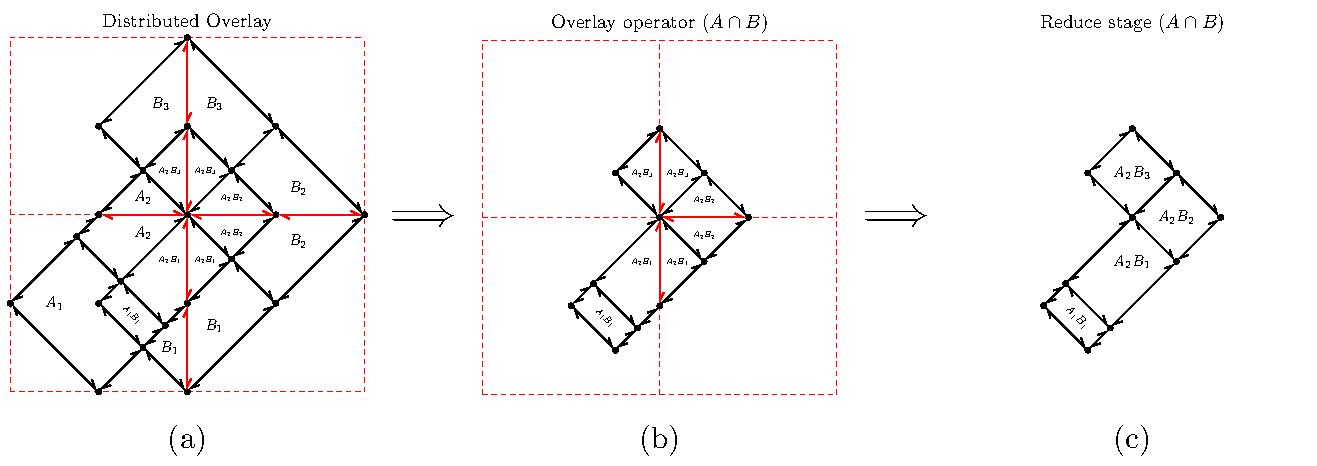
\includegraphics[width=\linewidth]{chapter2/overlay_operator.pdf}    
    \caption{Example of an overlay operator querying the distributed DCEL.} \label{fig:overlay_operator}
\end{figure}

\section{Overlay evaluation optimizations}\label{sec:alternative_methods}
We now focus on the different optimization aspects regarding the best approach to compute the boundaries of faces that expand different cells and how to mitigate the issues of layers with an unbalanced number of edges.
%\textbf{\color{red} TODO: I cannot asses how this section will be impacted by the new kd-tree partitioning, but we have to revise this.}

%\subsection{Optimizations for faces expanding cells}\label{sec:optimizing}
\subsection{Optimizations for faces spanning multiple cells}\label{sec:optimizing}

The naive reduce phase described above has the potential for a bottleneck since all faces, which can be a very large number, are sent to one worker node. 
From a distributed perspective, this process follows a typical MapReduce pattern. In the map phase, each worker node identifies and reports faces that are fully contained within its boundaries, as well as segments of faces that may need to be concatenated with segments reported by other nodes. These face segments are then sent to a master node, incurring communication costs as the master must wait for all nodes to report their segments. In the reduce phase, the master node groups the segments by face ID, sorts them, and concatenates the parts to form complete, closed faces.
One observation is that faces from different concatenated cells are in contiguous cells. This implies that faces from a particular cell will be combined with faces from neighboring cells. We will use this spatial proximity property to reduce the overhead in the central node.

We thus propose an alternative where an intermediate reduce processing step is introduced. In particular, the user can specify a level in the quadtree structure, measured as the depth from the root, that can be used to combine cells together. 
While it may be challenging to predetermine an optimal level, it can be estimated based on the input size or the number of partitions. Moreover, Section \ref{sec:overlay_optimization} offers recommendations for suitable values and alternative approaches.
Given level \textit{i}, the quadtree nodes in that level (at most $4^i$) will serve as intermediate reducers, collecting the faces from all the cells below that node. Note: level 0 corresponds to the root, which is the naive method where all the cells are sent to one node.

By introducing this intermediate step, it is expected that much of the reduce work can be distributed in a larger number of worker nodes. Nevertheless, there may be faces that cannot be completed by these intermediate reducers because they span the borders of the level $i$ nodes. Such faces still have to be evaluated in a master/root node.
From a Map-Reduce standpoint, this alternative functions similarly to the previous approach but introduces additional reduce operations at an intermediate level. However, this also introduces new synchronization points, as each intermediate reducer must wait for its workers to report potential face segments before processing them. The reducer then either reports completed faces or sends incomplete segments to the driver for further processing.

Clearly, picking the appropriate level is important. Choosing a level $i$, i.e., going to nodes lower in the quadtree structure, implies a larger number of intermediate reducers and, thus, higher parallelism. However, simultaneously, it increases the number of faces that would need to be evaluated by the master/root node. On the other hand, lowering $i$ reduces parallelism, but fewer faces will need to go to the master/root node.

We also examine another approach to deal with the bottleneck in the naive reduce phase. This approach re-partitions the faces using the label as the key. Such partitions represent small independent amounts of work since they only combine faces with the same label that are typically few. Partitions are then shuffled among the available nodes. The second approach effectively avoids the reduce phase; it has to account for the cost of the re-partitioning; however, as we will show in the experimental section, this cost is negligible.
From a distributed computing perspective, this alternative introduces a shuffle stage at the beginning, eliminating the need for a reduce operation. The shuffle ensures that all segments with the same face ID are placed in the same worker, allowing them to be processed and reported directly.

\subsection{Optimizing for unbalanced layers}\label{sec:unbalance}
During the overlay computation, finding the intersections between the half-edges is the most critical task. In many cases, the number of half-edges from each layer within a cell can be unbalanced; that is, one of the layers has many more half-edges than the other.

In our initial implementation, the input sets of half-edges within each cell were combined into a single dataset, initially ordered by the x-origin of each half-edge.
Then, a sweep-line algorithm is performed, scanning the half-edges from left to right (in the x-axis). This scanning takes time proportional to the total number of half-edges. However, if one layer has much fewer half-edges, the running time will still be affected by the cardinality of the larger dataset.

An alternative approach is to scan the larger dataset only for the x-intervals where we know that there are half-edges in the smaller dataset. To do so, we order the two input sets separately. We scan the smaller dataset in x-order and identify x-intervals occupied by at least one half-edge. For each x-interval, we then scan the larger dataset using the sweep-line algorithm. This focused approach avoids unnecessary scanning of the large dataset, for example, areas with no half-edges from the smaller dataset.
